\chapter{标题一}
\section{小节标题}
这是一个\textbf{加粗}和\textit{斜体}的文本。

这里是一个链接:\href{https://www.google.com}{Google}

我们引用了一些文献[\texttt{foo}],还有公式:$E = mc\textasciicircum{}2$

C\# 啊啊啊

段落结束。

\begin{itemize}
\item 无序列表
\item 无序列表是无序号的
\item 无序列表是个列表
\end{itemize}
\begin{enumerate}
\item 有序列表
\item 有序列表是有序号的
\item 有序列表是个列表
\end{enumerate}
\begin{figure}[h]
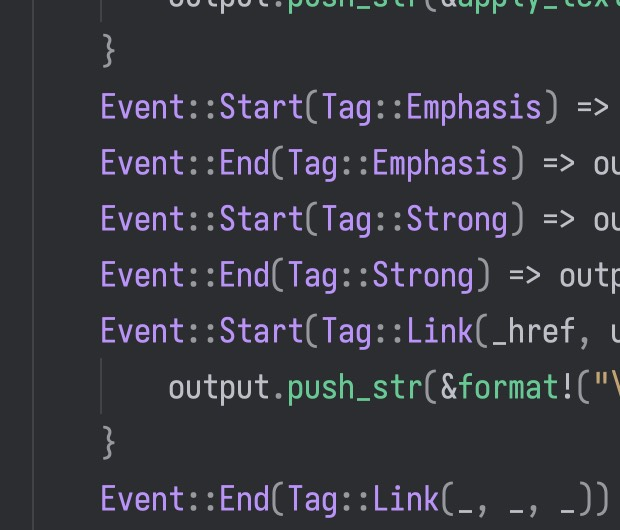
\includegraphics{images/test.jpg}
\caption{test image}
\label{fig:images/test.jpg}
\end{figure}


\textbackslash\{\}begin\{equation\}
\textbackslash\{\}frac\{1\}\{2\}\textbackslash\{\}mu
\textbackslash\{\}label\{eq:hhhhh\}
\textbackslash\{\}end\{equation\}

